\documentclass{standalone}
\usepackage{tikz}
\usetikzlibrary{patterns, positioning}

\begin{document}
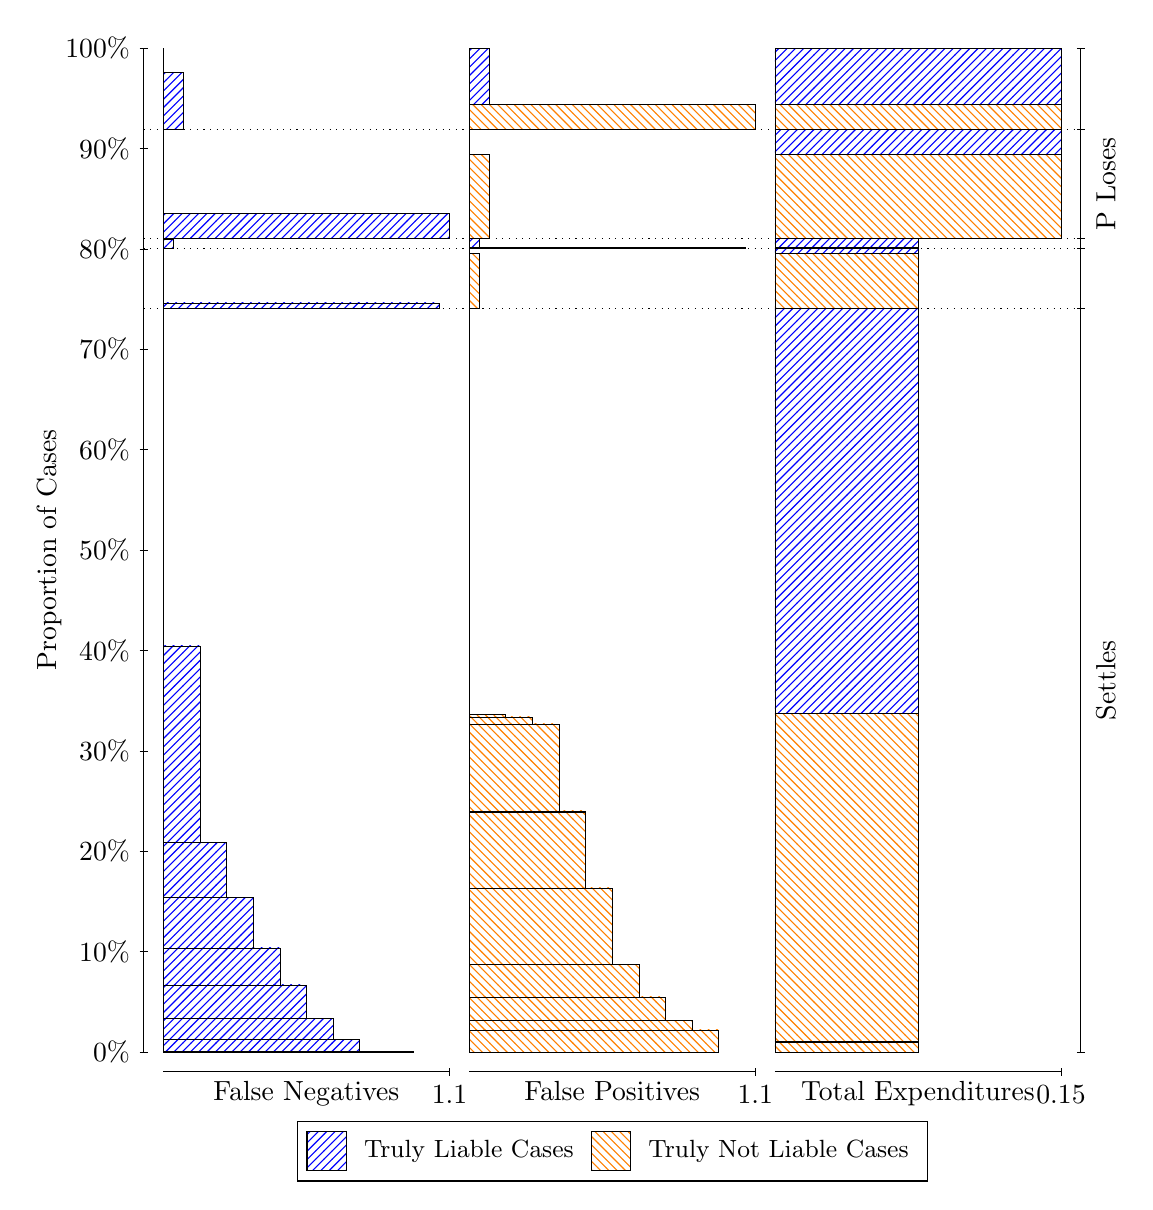
\begin{tikzpicture}
\draw[black, very thin] (1.5,1.75) -- (1.5,14.5);
\node[rotate=90, anchor=center] at (0.3, 8.125) {Proportion of Cases};
\draw[black, very thin] (1.45,1.75) -- (1.55,1.75);
\node[anchor=east] at (1.45, 1.75) {0\%};
\draw[black, very thin] (1.45,3.025) -- (1.55,3.025);
\node[anchor=east] at (1.45, 3.025) {10\%};
\draw[black, very thin] (1.45,4.3) -- (1.55,4.3);
\node[anchor=east] at (1.45, 4.3) {20\%};
\draw[black, very thin] (1.45,5.575) -- (1.55,5.575);
\node[anchor=east] at (1.45, 5.575) {30\%};
\draw[black, very thin] (1.45,6.85) -- (1.55,6.85);
\node[anchor=east] at (1.45, 6.85) {40\%};
\draw[black, very thin] (1.45,8.125) -- (1.55,8.125);
\node[anchor=east] at (1.45, 8.125) {50\%};
\draw[black, very thin] (1.45,9.4) -- (1.55,9.4);
\node[anchor=east] at (1.45, 9.4) {60\%};
\draw[black, very thin] (1.45,10.675) -- (1.55,10.675);
\node[anchor=east] at (1.45, 10.675) {70\%};
\draw[black, very thin] (1.45,11.95) -- (1.55,11.95);
\node[anchor=east] at (1.45, 11.95) {80\%};
\draw[black, very thin] (1.45,13.225) -- (1.55,13.225);
\node[anchor=east] at (1.45, 13.225) {90\%};
\draw[black, very thin] (1.45,14.5) -- (1.55,14.5);
\node[anchor=east] at (1.45, 14.5) {100\%};

\draw[black, very thin] (13.4,1.75) -- (13.4,14.5);
\draw[black, very thin] (13.35,1.75) -- (13.45,1.75);
\node[anchor=west] at (13.35, 1.75) {};
\draw[black, very thin] (13.35,11.195) -- (13.45,11.195);
\node[anchor=west] at (13.35, 11.195) {};
\draw[black, very thin] (13.35,11.957) -- (13.45,11.957);
\node[anchor=west] at (13.35, 11.957) {};
\draw[black, very thin] (13.35,12.081) -- (13.45,12.081);
\node[anchor=west] at (13.35, 12.081) {};
\draw[black, very thin] (13.35,13.467) -- (13.45,13.467);
\node[anchor=west] at (13.35, 13.467) {};
\draw[black, very thin] (13.35,14.5) -- (13.45,14.5);
\node[anchor=west] at (13.35, 14.5) {};

\draw[black, very thin, pattern color=blue, pattern=north east lines] (1.75,1.75) rectangle (4.9186,1.7526);
\draw[black, very thin, pattern color=blue, pattern=north east lines] (1.75,1.7526) rectangle (4.5806,1.7611);
\draw[black, very thin, pattern color=blue, pattern=north east lines] (1.75,1.7611) rectangle (4.2426,1.9078);
\draw[black, very thin, pattern color=blue, pattern=north east lines] (1.75,1.9078) rectangle (3.9047,2.1779);
\draw[black, very thin, pattern color=blue, pattern=north east lines] (1.75,2.1779) rectangle (3.5667,2.6025);
\draw[black, very thin, pattern color=blue, pattern=north east lines] (1.75,2.6025) rectangle (3.2287,3.0728);
\draw[black, very thin, pattern color=blue, pattern=north east lines] (1.75,3.0728) rectangle (2.8907,3.7107);
\draw[black, very thin, pattern color=blue, pattern=north east lines] (1.75,3.7107) rectangle (2.5527,4.4162);
\draw[black, very thin, pattern color=blue, pattern=north east lines] (1.75,4.4162) rectangle (2.2147,6.9079);
\draw[black, very thin, pattern color=orange, pattern=north west lines] (1.75,6.9079) rectangle (1.75,11.195);
\draw[black, very thin, pattern color=blue, pattern=north east lines] (1.75,11.195) rectangle (5.2566,11.264);
\draw[black, very thin, pattern color=orange, pattern=north west lines] (1.75,11.264) rectangle (1.75,11.957);
\draw[black, very thin, pattern color=blue, pattern=north east lines] (1.75,11.957) rectangle (1.8767,12.07);
\draw[black, very thin, pattern color=orange, pattern=north west lines] (1.75,12.07) rectangle (1.75,12.081);
\draw[black, very thin, pattern color=blue, pattern=north east lines] (1.75,12.081) rectangle (5.3833,12.396);
\draw[black, very thin, pattern color=orange, pattern=north west lines] (1.75,12.396) rectangle (1.75,13.467);
\draw[black, very thin, pattern color=blue, pattern=north east lines] (1.75,13.467) rectangle (2.0035,14.187);
\draw[black, very thin, pattern color=orange, pattern=north west lines] (1.75,14.187) rectangle (1.75,14.5);
\draw[black, very thin, pattern color=orange, pattern=north west lines] (5.6333,1.75) rectangle (8.8019,2.03);
\draw[black, very thin, pattern color=orange, pattern=north west lines] (5.6333,2.03) rectangle (8.464,2.1558);
\draw[black, very thin, pattern color=orange, pattern=north west lines] (5.6333,2.1558) rectangle (8.126,2.4485);
\draw[black, very thin, pattern color=orange, pattern=north west lines] (5.6333,2.4485) rectangle (7.788,2.858);
\draw[black, very thin, pattern color=orange, pattern=north west lines] (5.6333,2.858) rectangle (7.45,3.8339);
\draw[black, very thin, pattern color=orange, pattern=north west lines] (5.6333,3.8339) rectangle (7.112,4.7956);
\draw[black, very thin, pattern color=orange, pattern=north west lines] (5.6333,4.7956) rectangle (7.112,4.8115);
\draw[black, very thin, pattern color=orange, pattern=north west lines] (5.6333,4.8115) rectangle (6.774,5.9171);
\draw[black, very thin, pattern color=orange, pattern=north west lines] (5.6333,5.9171) rectangle (6.436,6.0058);
\draw[black, very thin, pattern color=orange, pattern=north west lines] (5.6333,6.0058) rectangle (6.0981,6.0369);
\draw[black, very thin, pattern color=blue, pattern=north east lines] (5.6333,6.0369) rectangle (5.6333,11.195);
\draw[black, very thin, pattern color=orange, pattern=north west lines] (5.6333,11.195) rectangle (5.7601,11.888);
\draw[black, very thin, pattern color=blue, pattern=north east lines] (5.6333,11.888) rectangle (5.6333,11.957);
\draw[black, very thin, pattern color=orange, pattern=north west lines] (5.6333,11.957) rectangle (9.1399,11.968);
\draw[black, very thin, pattern color=blue, pattern=north east lines] (5.6333,11.968) rectangle (5.7601,12.081);
\draw[black, very thin, pattern color=orange, pattern=north west lines] (5.6333,12.081) rectangle (5.8868,13.152);
\draw[black, very thin, pattern color=blue, pattern=north east lines] (5.6333,13.152) rectangle (5.6333,13.467);
\draw[black, very thin, pattern color=orange, pattern=north west lines] (5.6333,13.467) rectangle (9.2667,13.78);
\draw[black, very thin, pattern color=blue, pattern=north east lines] (5.6333,13.78) rectangle (5.8868,14.5);
\draw[black, very thin, pattern color=orange, pattern=north west lines] (9.5167,1.75) rectangle (11.333,1.8698);
\draw[black, very thin, pattern color=blue, pattern=north east lines] (9.5167,1.8698) rectangle (11.333,1.8809);
\draw[black, very thin, pattern color=orange, pattern=north west lines] (9.5167,1.8809) rectangle (11.333,6.048);
\draw[black, very thin, pattern color=blue, pattern=north east lines] (9.5167,6.048) rectangle (11.333,11.195);
\draw[black, very thin, pattern color=orange, pattern=north west lines] (9.5167,11.195) rectangle (11.333,11.888);
\draw[black, very thin, pattern color=blue, pattern=north east lines] (9.5167,11.888) rectangle (11.333,11.957);
\draw[black, very thin, pattern color=orange, pattern=north west lines] (9.5167,11.957) rectangle (11.333,11.968);
\draw[black, very thin, pattern color=blue, pattern=north east lines] (9.5167,11.968) rectangle (11.333,12.081);
\draw[black, very thin, pattern color=orange, pattern=north west lines] (9.5167,12.081) rectangle (13.15,13.152);
\draw[black, very thin, pattern color=blue, pattern=north east lines] (9.5167,13.152) rectangle (13.15,13.467);
\draw[black, very thin, pattern color=orange, pattern=north west lines] (9.5167,13.467) rectangle (13.15,13.78);
\draw[black, very thin, pattern color=blue, pattern=north east lines] (9.5167,13.78) rectangle (13.15,14.5);
\draw[black, dotted] (1.5,11.195) -- (13.4,11.195);
\draw[black, dotted] (1.5,11.957) -- (13.4,11.957);
\draw[black, dotted] (1.5,12.081) -- (13.4,12.081);
\draw[black, dotted] (1.5,13.467) -- (13.4,13.467);
\draw[black, very thin] (1.75,1.5) -- (5.3833,1.5);
\node[anchor=north] at (3.5667, 1.5) {False Negatives};
\draw[black, very thin] (5.3833,1.45) -- (5.3833,1.55);
\node[anchor=north] at (5.3833, 1.45) {1.1};

\draw[black, very thin] (5.6333,1.5) -- (9.2667,1.5);
\node[anchor=north] at (7.45, 1.5) {False Positives};
\draw[black, very thin] (9.2667,1.45) -- (9.2667,1.55);
\node[anchor=north] at (9.2667, 1.45) {1.1};

\draw[black, very thin] (9.5167,1.5) -- (13.15,1.5);
\node[anchor=north] at (11.333, 1.5) {Total Expenditures};
\draw[black, very thin] (13.15,1.45) -- (13.15,1.55);
\node[anchor=north] at (13.15, 1.45) {0.15};

\node[black, centered, rotate=90] at (13.72, 6.4724) {Settles};


\node[black, centered, rotate=90] at (13.72, 12.774) {P Loses};


\draw (7.449999999999999,1.5) node[draw=none] (baseCoordinate) {};
\begin{scope}[align=center]
        \matrix[scale=0.5, draw=black, below=0.5cm of baseCoordinate, nodes={draw}, column sep=0.1cm]{
            \node[rectangle, draw, minimum width=0.5cm, minimum height=0.5cm, pattern=north east lines, pattern color=blue] {}; &
            \node[draw=none, font=\small] (B) {Truly Liable Cases}; &
            \node[rectangle, draw, minimum width=0.5cm, minimum height=0.5cm, pattern=north west lines, pattern color=orange] {}; &
            \node[draw=none, font=\small] (B) {Truly Not Liable Cases}; \\
            };
\end{scope}

\end{tikzpicture}
\end{document}